% !TEX root=../main.tex
\chapter{Background}
\renewcommand{\baselinestretch}{\mystretch}
%\setlength{\parindent}{0pt}
\PARstart{T}{his} chapter is a summary of previous research based on audio data. Three main aspects of work were focused on where the performance has been improved. Firstly, different feature extract methods based on audio data are compared in previous studies. Two classical representation will be introduced, namely STFT and MFCCs. Afterwards, statistical learning and deep neuronal network models applied to audio data mining are compared in Section 2.2. Finally, studies of data pre-processing methods including noise reduction and augmentation are discussed. 
\section{Audio Feature Extraction}
When Welch~\cite{welch1967use} proposed a fast Fourier transform algorithm, namely short-time Fourier transform (STFT), efficient estimation of power spectra could be used on record analysis. He suggested segmental processing of the whole record and moving the window with possible overlapping, which can not only modify periodogram by averaging but also reduce computational complexity. Afterwards, Davis and Mermelstein~\cite{davis1980comparison} introduced Mel-frequency cepstral coefficients (MFCC) based on STFT. Due to the linear characteristic of Fourier transform, MFCCs are perceptual features which mimic received signal by the cochlea, aiming to enhance signal with significant contribution in phonetic detection. They firstly applied triangular mel-filters to scale spectrogram, then taking logarithm and discrete cosine transform (DCT) to calculate significant cepstral coefficients. \par
Lippends et al.~\cite{lippens2004comparison} compared performances of an auditory model and MFCC features in music genre classification task. They extracted 4 features from STFT and first 5 Mel-frequency cepstral coefficients classified by Gaussian Mixture Model (GMM), which shows that the auditory model has no outstanding accuracy than standard MFCC. Moreover, 12 identified MFCCs are used on recognition of anuran species~\cite{bedoya2014automatic}, achieving average accuracy in 99.61\% of all six species. However, MFCCs are not robust for the noisy environment, resulting in utilizing mel-spectrogram as representations. Choi et al.~\cite{choi2016automatic} compared STFT, MFCC and Mel-spectrogram (with accuracy 84.6\%, 86.2\% and 89.4\% respectively) using four layers of fully convolutional neural networks (FCN) on automatic tagging MagnaTagATune dataset. Similar work was studied in~\cite{huzaifah2017comparison} with additional fast
wavelet transform (FWT) and continuous wavelet transform
(CWT) as comparisons. He proved that mel-spectrogram still achieved significant performance on UrbanSound8K dataset among variations of settings, although STFT and CWT had some outstanding results on some models.\par
MFCC and mel-spectrogram are broadly used on automated species detection as well. Clemin et al.~\cite{clemins2003application} studied in recognizing African elephants sound based on GMM in 2003, resulting accuracies of 83.8\% for call and 88.1\% for identification.
Feature comparison of log-magnitude spectrogram using CNN and log-mel band energy using CRNN were studied in \cite{cakir2017convolutional}, improving the accuracy in 3\%. They stated that log-mel band energy makes bird sound more distinguishable. Another application on insect sound recognition was studied by~\cite{le2011insect}, using Probabilistic Neural Network (PNN) based on Bayesian classifiers. Although the identification accuracy is over 92\%, the method of selecting noise-free sections still introduced limitations in generalisation.

In summary, approaches of feature extraction significantly determine the performance of audio detection problems. By transforming time-series into cepstrum coefficients or spectrogram, the feature dimensions are reduced to a large extent. MFCCs present distinction on compressive representations which uses 12-20 coefficients as features~\cite{lippens2004comparison,le2011insect,clemins2003application}. Hence, it is beneficial to the linear statistical model, such as hidden Markov models and Gaussian Mixture Model. Mel-spectrogram is still an alternative with the advantage of noisy robustness. Therefore, mel-spectrogram is a suitable representation for deep learning, containing more distinguishable features.
\section{Automated Recognition Models}
In the past decade, hidden Markov models (HMM) and Gaussian Mixture model (GMM) were based on mathematical statistics. HMM aims to use observable data to predict the hidden feature based on the Markov process, for example predict event label with giving time-series signal. The property of the Markov process is that hidden variables of current time $s(t)$ only depends on previous time $s(t-1)$. Therefore, this property determined the suitability of speech recognition~\cite{rabiner1989tutorial} whose signals have relevance among context. Research based on HMM in antbirds recognition was studied by Vlad et al.~\cite{trifa2008automated}, who used optional MFCC features including energy, delta coefficients, acceleration. They found that varying estimated states from 5 to 15 could degrade performance dropped from 94.6\% to 82.5\%.\par
GMM is another general model since most of data in real life are subject to Gaussian distribution. Thus, using GMM by setting several mixtures can estimate the data distribution. Data can be considered as same label if they have a similar distribution. Brown \& Smaragdis~\cite{brown2009hidden} compared both GMM and HMM model on marine call types classification. The results proved that both these statistical models are powerful for acoustic classification of killer whales.
Zhao~\cite{zhao2017automated} used a sophisticated method of modelling log-band energy in order to automatically segment activities. The GMM-based model with two mixtures can capture both high-energy frames and low-energy frames, selecting the cross point as the threshold. Therefore, discriminative features of bird were selected, resulting in improved robustness of SVM to classify.

Both HMM and GMM are based on expectation maximum algorithm to estimate the probability of unknown parameters. Nevertheless, HMM takes temporal context into account, whereas GMM treats the whole signal as a unique spectral individual~\cite{brown2009hidden}. Comparing studies in~\cite{clemins2003application,trifa2008automated,zhao2017automated}, MFCCs were often used as features of GMM and HMM model. The reason may be that MFCCs largely compress the feature representations which make the statistical model easy to train. However, the mel-spectrogram can be consider as an effective alternative when using powerful models like CNN.

In recent years, deep learning has been rapidly developed on audio recognition since it can learn more effective features from input. Since VGGNet has outstanding performance on Large Vocabulary Continuous Speech Recognition (LVCSR)~\cite{sercu2016very}, convolutional neural network successfully applied on Acoustic Event Detection (AED) 80.3\% with accuracy~\cite{takahashi2016deep}. 
Moreover, Cakir et al.~\cite{cakir2017convolutional} proposed that using converlutional recurrent neural network (CRNN) with log-mel band energy as features improved the accuracy up to 88.5\% on bird event detection. Continue to bird detection, Grill et al.~\cite{8081512} designed two types of CNN architectures to detect the presence of bird call. General architecture designed with each convolutional layer following a pooling layer and using three dense layers, while local architecture used convolutional layers instead of dense layer transforming into a one-dimensional sequence and selected the maximum. Table \ref{tabel:summarymodel} makes a summary of these researches with different models and feature extraction methods. The types of recognition tasks and overall accuracy are recorded as well.
\begin{table}[htp]
\centering
\caption{Summary of models and feature extraction methods on species detection}
\label{tabel:summarymodel}
\begin{tabular}{ccccc}
\hline
Model& Species& Task& Feature& Accuracy(\%)\\
\hline
GMM& Elephant (2003)& Detection&MFCC& 83.8~\cite{clemins2003application}\\
HMM& Antbird (2008)& Detection&MFCC& 94.6~\cite{trifa2008automated}\\
GMM+HMM& Whales (2009)&Classification& MFCC & 92~\cite{brown2009hidden}\\
GMM+SVM& Bird (2017)& Classification& MFCC& $>$ 90~\cite{zhao2017automated}\\
PNN& Insect (2011)& Identification& MFCC& 92.44~\cite{le2011insect}\\
CNN& Bird (2017)&Detection& Log-spectrogram& 85.5~\cite{cakir2017convolutional}\\
CRNN& Bird (2017)& Detection& Log-mel energy
& 88.5 \cite{cakir2017convolutional}\\
CNN& Bat (2018)& Detection& STFT
& 89.6 \cite{batdetect18}\\
\hline
\end{tabular}
\end{table}
\section{Processing on Audio data}
For obtaining higher performance for species detection, several data processing method can be applied in order to improve the feature representation instead of inputting raw data. There are two main method that significant improve the performance of CNN model, specifically noise reduction and data augmentation. Noise reduction can enhance the region of interests (ROIs), making the call more distinct. Augmentation can increase the variation for training if only small number of data can be collected.

Generally, the acoustic recording is unavoidably introduced disturbance by the high-level noise, which related to the habitats that recording devices installed. Thus, environmental sounds have significant effects on the estimation of species' activity, introducing detection bias. As the denoising method implemented in~\cite{aide2013real,batdetect18}, regions of interests were enhanced with reducing the noise level. They applied spectral subtraction method which removed the mean amplitude in each frequency band as shown in \ref{fig:batnoise}. The level of background noise was suppressed to a large extent and removing the additive noise. Thus, the CNN model can effectively classify the foreground echo and the background noise with a high output probability of the presence of call. 
\begin{figure}[htp]
\centering
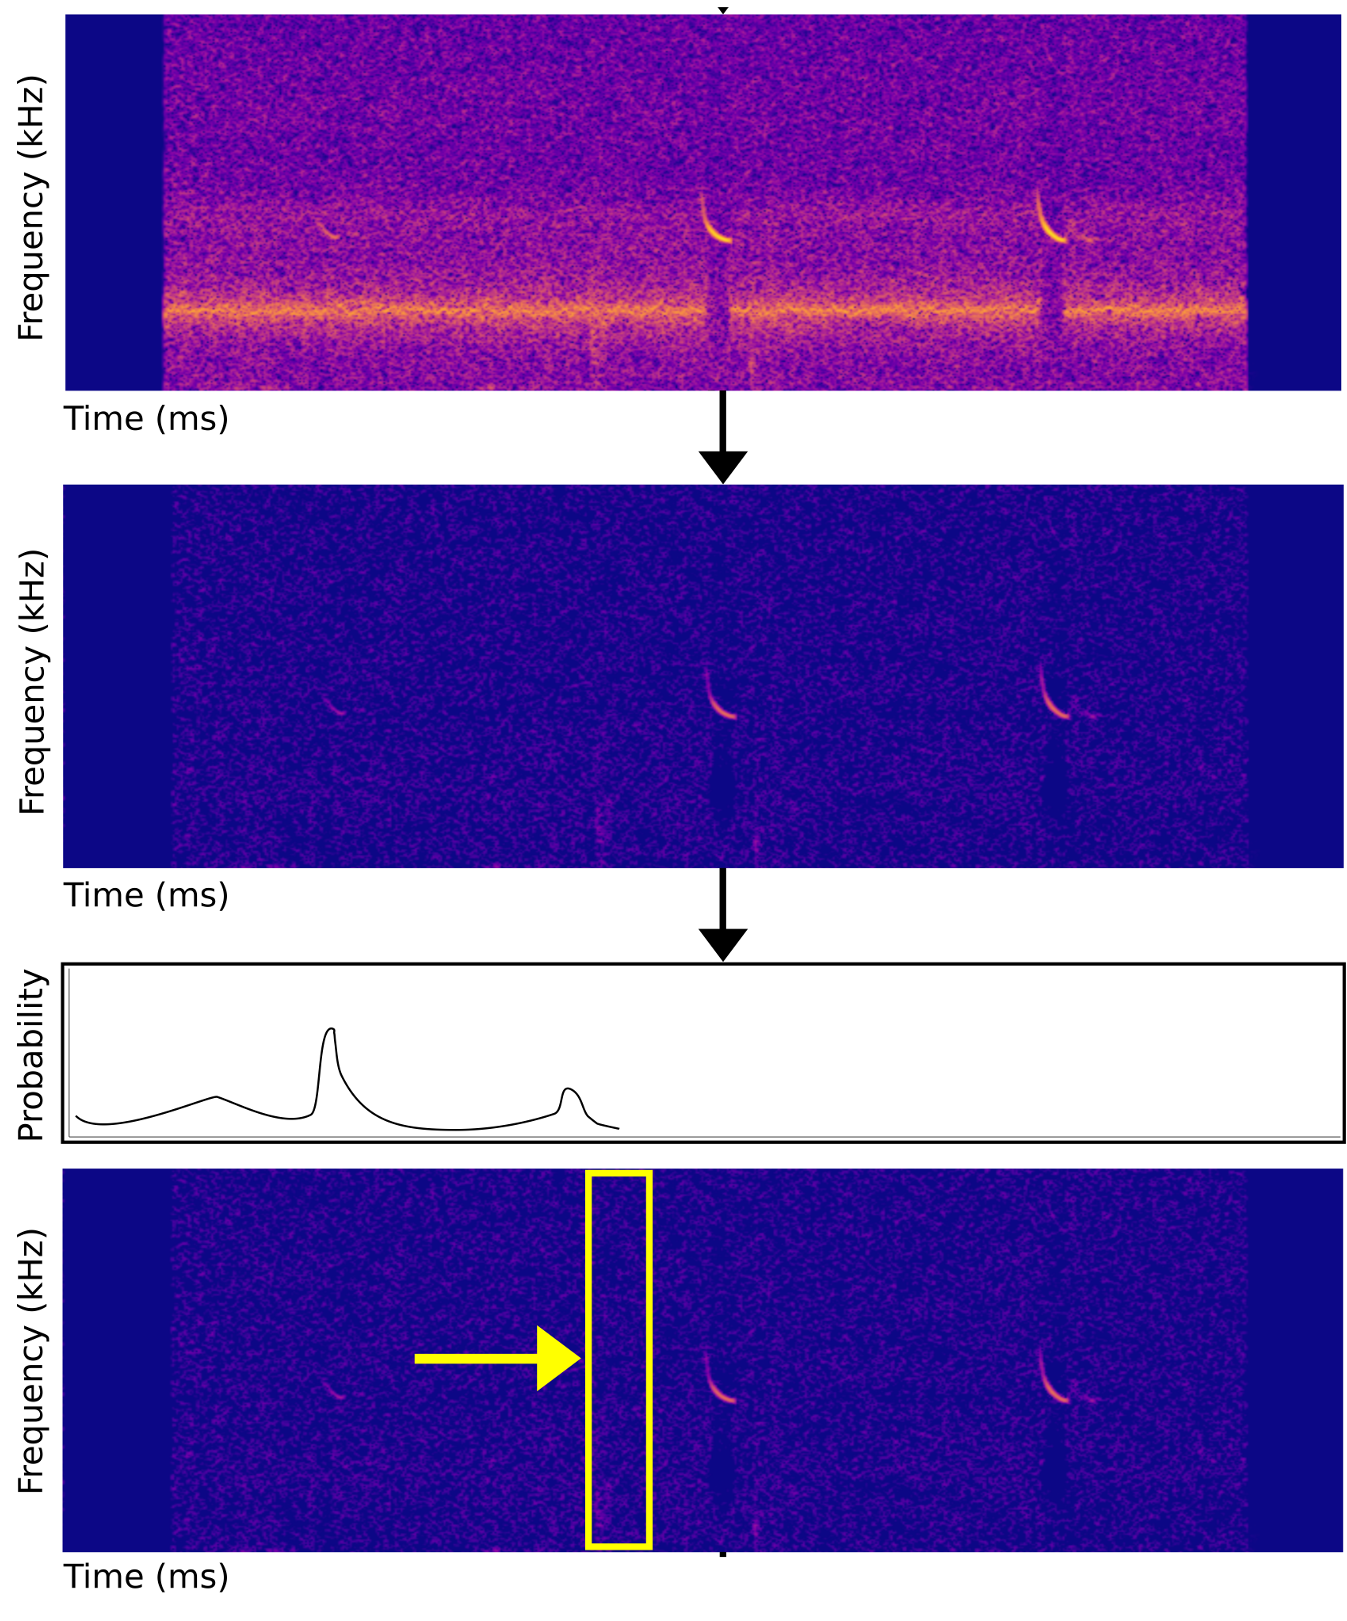
\includegraphics[scale=0.8]{Figs/chap2/batnoise.png}
\caption[Noise reduction of bat call]{Noise reduction of bat call in spectrogram representation~\cite{batdetect18}}
\label{fig:batnoise}
\end{figure}

Minimum mean-square error log-spectral amplitude (MMSE-LSA) estimator is another effective algorithm, which has been extensively implemented in automatic speech recognition (ASR) systems. Kim \& Rose~\cite{kim2002cepstrum} proposed a way of combining model based on MMSE-LSA to decompose noise and speech signal in the cepstral domain. Via combining MMSE-LSA technique with HMM model, the robustness of MFCCs is significantly increased. The MMSE-LSA estimator highly depends on a prior signal to noise ratio (SNR), which is estimated in the presence of non-speech region. Hence, \textit{a prior} SNR estimator based on CNN is introduced by \cite{nicolson2019deep}. The experiments by using deep learning showed the quality and intelligibility scores are much better than masking and mapping methods. However, there are fewer studies applied the MMSE-LSA for species detection tasks. In this project, I applied MMSE-LSA on 'whinny' calls to evaluate the performance.

Augmenting data is a necessary approach for model training especially on a small dataset. Takahashi et al.~\cite{takahashi2016deep} introduced a new augmentation method for audio event classification since the number of audio in each class is small. It is called Equalized Mixture Data Augmentation (EMDA) which mixes two different audio segments in the same class to synthesize new data. Moreover, he further modified the frequency characteristics by enhancing or disturbing a particular frequency band. By using augmentation, the accuracy was improved in 10\% compared with the original dataset. Other augmentation methods are compared in \cite{sprengel2016audio} as well for bird sounds identification, namely adding white noise, pitch shift, time shift and combining same class. He proved that time-shift took a large impact on performance, resulting in accuracy decreasing 3\% without applying time-shift. 


